% Log4Tailer: A multicolored python tailer for log4J logs
% Copyright (C) 2011 Jordi Carrillo Bosch
% 
% Permission is granted to copy, distribute and/or modify this
% document under the terms of the GNU Free Documentation License,
% Version 1.3 or any later version published by the Free Software
% Foundation; with no Invariant Sections, no Front-Cover Texts and
% no Back-Cover Texts.  A copy of the license is included in the
% section entitled "GNU Free Documentation License".

\documentclass[a4paper, twoside]{article}
%\documentclass[letterpaper]{article}
%\usepackage{lmodern}
% for non-serified font
%\renewcommand*\familydefault{\sfdefault}
\usepackage[usenames, dvipsnames]{xcolor}
\usepackage[tikz]{bclogo}
\usepackage{framed}
\usetikzlibrary[petri,arrows,decorations.pathmorphing,backgrounds,positioning,fit,shapes]
\usepackage[hmargin=2.5cm,vmargin=2.5cm]{geometry}
\usepackage{verbatim}
\usepackage{epigraph}
\usepackage{wrapfig}
\usepackage{graphicx}
\usepackage[stable]{footmisc}
\usepackage{hyperref}
\usepackage{booktabs}
\usepackage{colortbl}
%\usepackage[colorinlistoftodos, textwidth=4cm, shadow, disable]{todonotes} 
\usepackage[colorinlistoftodos, textwidth=2cm]{todonotes} 

% specific acrobat reader settings
\hypersetup{colorlinks=true,
            linkcolor=blue,
            filecolor=blue,%magenta,
            pagecolor=blue,%red,
            urlcolor=blue,%cyan,
            citecolor=blue,
            pdfauthor={Jordi Carrillo},%
			pdftitle={Log4Tailer User's Guide},%
			pdfborder={0 0 0},%
			pdfstartview={FitH},%
			bookmarksnumbered=true,%
			bookmarks=true,%
			pdftex}
%\usepackage[pdftex,pdfborder={0 0 0},pdfstartview={FitH},bookmarksnumbered=true]{hyperref}
%\usepackage{makeidx}
%\makeindex

\newenvironment{cmd}{\fontsize{9pt}{11}\color{blue}\verbatim} {\endverbatim}
\newenvironment{outlog}{\fontsize{9pt}{11}\color{red}\verbatim} {\endverbatim}
\newenvironment{filec}{\fontsize{9pt}{11}\color{black}\verbatim} {\endverbatim}
\newenvironment{test}{\begin{center}}{\end{center}}

\definecolor{fbase}{gray}{0.95}
\newenvironment{gbar}[1]{%
\def\FrameCommand {{\color{#1}\vrule width 3 pt}\colorbox{fbase}}%
\MakeFramed {\advance\hsize-\width \FrameRestore}}%
{\endMakeFramed}

\author{Jordi Carrillo}
\title{User Guide to Log4Tailer}

\newcommand{\logftailertitle}{\textbf{\textcolor{black}{L}\textcolor{red}{o}%
\textcolor{Violet}{g}4\textcolor{green}{T}\textcolor{magenta}{ail}\textcolor{red}{er}}}
\newcommand{\logftailer}{\textbf{\textcolor{black}{A}\textcolor{red}{l}%
\textcolor{Violet}{e}\textcolor{green}{r}\textcolor{magenta}{t}\textcolor{red}{a}}}

\newcommand{\emphlogtrace}[1]{\vspace{0.2cm}\newline\indent\colorbox{red}{\textbf{#1}}\newline\vspace{0.2cm}}

%\usepackage{sectsty}
%\usepackage{float}
%\floatstyle{plain}
%\newfloat{picture}{htp}{pictures}
%\floatname{picture}{Screenshot}
%\def\pictureautorefname{screenshot}

\usepackage[figure]{hypcap}

\usepackage{colortbl}



%FIXME needs some cleanup in here
\newcommand{\contentsrule}[1]{{\color{blue}\sectionrule{3ex}{3pt}{-2ex}{1pt}{#1}}}
\renewcommand{\contentsname}{{\color{cadetblue}\rule{\textwidth}{2pt}}\\\logftailer{}'s %
Contents\\\rule[1ex]{\textwidth}{1pt}}


\definecolor{myblue}{rgb}{0.8,0.8,1}
\makeatletter\newenvironment{codeexample}{%
   \vspace{0.15cm}\noindent\begin{lrbox}{\@tempboxa}\begin{minipage}{0.98\columnwidth}\setlength{\parindent}{1em}}{\end{minipage}\end{lrbox}%
   \colorbox{lowgreen}{\usebox{\@tempboxa}}\vspace{0.15cm}
}\makeatother

% \usepackage{float}
% \floatstyle{boxed} 
% \restylefloat{figure}

\definecolor{myorange}{rgb}{1,0.8,0}
\makeatletter\newenvironment{config}{%
   \vspace{0.2cm}\noindent\begin{lrbox}{\@tempboxa}\begin{minipage}{0.98\textwidth}\setlength{\parindent}{1em}}{\end{minipage}\end{lrbox}%
   \colorbox{lowgreen}{\usebox{\@tempboxa}}\vspace{0.2cm}
}\makeatother

\newcommand{\logoheader}{\begin{tikzpicture}
    \draw[fill=violet] (0,0) ellipse [x radius=0.5cm,y radius=0.4cm];
    \draw (-0.5,0) -- (0.5,0);
    \draw (0,-0.4) -- (0,0.4);
    \draw[fill=red] (-0.06,0.05) circle (0.2cm);
    \draw[fill=red, nearly opaque] (-0.06,0.05) circle (0.3cm);
    \draw[fill=yellow] (-0.05,0.05) circle (0.05cm);
\end{tikzpicture}}


\newcommand{\logo}{\begin{tikzpicture}
    \draw[fill=violet] (0,0) ellipse [x radius=1cm,y radius=0.8cm];
    \draw (-1,0) -- (1,0);
    \draw (0,-0.8) -- (0,0.8);
    \draw[fill=red] (-0.12,0.1) circle (0.4cm);
    \draw[fill=red, nearly opaque] (-0.12,0.1) circle (0.6cm);
    \draw[fill=yellow] (-0.1,0.1) circle (0.1cm);
\end{tikzpicture}}

\usepackage{fancyhdr}
\fancyhead{}
\fancyfoot{}
\fancyhead[RO,LE]{\logftailer{} Project} % \logoheader}
\fancyhead[LO,RE]{\nouppercase\leftmark} % \logoheader}
\fancyfoot[C]{\thepage}
%\rhead{\nouppercase{\leftmark}}
%\lhead{\nouppercase{\leftmark}}

%\renewcommand{\headrulewidth}{0.4pt}
%\renewcommand{\footrulewidth}{0pt}

\begin{document}

% Title page
% Log4Tailer: A multicolored python tailer for log4J logs
% Copyright (C) 2008 Jordi Carrillo Bosch
% 
% Permission is granted to copy, distribute and/or modify this
% document under the terms of the GNU Free Documentation License,
% Version 1.3 or any later version published by the Free Software
% Foundation; with no Invariant Sections, no Front-Cover Texts and
% no Back-Cover Texts.  A copy of the license is included in the
% section entitled "GNU Free Documentation License".

\definecolor{darkgreen}{rgb}{0.25,0.25,0.112}
\definecolor{aliceblue}{rgb}{0.941176,0.972549,1}
\definecolor{cadetblue}{rgb}{0.372549,0.619608,0.627451}
\definecolor{ghostwhite}{rgb}{0.972549,0.972549,1}
\definecolor{kaki}{rgb}{0.941176,0.901961,0.54902}
\definecolor{blueblackmine}{rgb}{0.65625,0,0.65625}
\definecolor{greeny}{rgb}{0.92,0.92,1}
\thispagestyle{empty}
\colorlet{lowgreen}{green!50!orange!25!yellow!15}
%\pagecolor{aliceblue}
%\pagecolor{greeny}
%\pagecolor{lowgreen}
\definecolor{lightblue}{rgb}{0.8352, 0.8823, 0.86666}
\pagecolor{aliceblue}
\vbox{}
  \vskip3pt plus 2fill
\noindent
{\Huge\alerta{} \textbf{Project}}\\
\logo
%\includegraphics{alerta35.png}
%\emph{Not just a simple log tailer}
%\vskip2pt plus 1fill
%\begin{flushright}
%\includegraphics{log4tailerdoc.png}
%\end{flushright}
% Some tikz fun ;-)
\begin{center}
\begin{tikzpicture}
[node distance=1.3cm,place/.style={circle,draw=blue!50,fill=blue!20,thick,
               inner sep=5pt,minimum size=6mm},
 transition/.style={rectangle,draw=black!50,fill=black!20,thick,
                    inner sep=5pt,minimum size=6mm}]

\node[place, fill=green] (begin) {Logs};
\node[transition] (stdout) [right=of begin] {{\color{red}\textbf{STDOUT}}};
\node[place] (executor) [above= of stdout] {{\color{magenta}\textbf{Executor}}};

\node[place] (mail) [above=of executor, label={[label distance=0.5cm]above:\Large\textbf{Notifications}}] {Email};
%\node[cloud, fill=white] (poster) [left= of mail] {{\color{blue}\textbf{Poster}}};
\node[place, very thick, draw=green, fill=white] (log4tailer) [left=of
 begin, %,label=below:\emph{Not just a simple log tailer},
pin={[pin edge={<-, blue,thick}]180:\textbf{Configuration File}}] {\Large \logftailer{}};

\node[place, draw=red, thick, fill=yellow!20,node distance=2cm] (reporting) [below= of log4tailer] {\textbf{Reporting}};

%\node[place, draw=red, thick, fill=yellow!20,node distance=2cm] (reporting) at (-8, -4) {\textbf{Reporting}};
\node[place] (reportingemail) [below= of reporting] {Email};
\node[transition] (reportingstdout) [right= of reportingemail] {{\color{red}\textbf{STDOUT}}};
\node[place, fill=red!50] (reportingfile) [left= of reportingemail] {File};
\node[place, draw=red, fill=red] (cornermark) [below=of stdout] {\textbf{cornerMark}};
\node[place, fill=orange] (inactivity) [below=of cornermark] {inactivity};
\node[place, fill=yellow] (filter) [below=of inactivity] {filter};

\draw [->, decorate, blue, thick, decoration={snake}] (log4tailer) -- (begin);
\draw [->] (begin) to [out=90, in=180] node[sloped, above, midway] {\textbf{notify}} (mail);%.. controls +(up:5mm) .. (mail.west);
\draw[->, red, thick] (begin) to [out=45, in=180] (executor);
\draw [->, draw=blue, thick] (begin.east) -- (stdout.west);
\draw [->] (begin) to [out=270,in=130] (cornermark);  %+(down:2mm) and +(up:5mm) .. (cornermark.west);
\draw [->] (begin) to [out=270,in=140] (inactivity);%.. controls +(down:5mm) .. (inactivity.west);
\draw [->] (begin) to [out=270,in=135] (filter);%.. controls +(down:5mm) .. (inactivity.west);

\draw [->, decorate, red, thick, decoration={snake}] (log4tailer) to [out=270,in=90] (reporting);%.. controls +(down:5mm) .. (inactivity.west);

\draw [->, decorate, blue, thick, decoration={snake}] (log4tailer) to [out=285,in=75] (reporting);%.. controls +(down:5mm) .. (inactivity.west);

\draw [->, decorate, orange, thick, decoration={snake}] (log4tailer) to [out=255,in=105] (reporting);%.. controls +(down:5mm) .. (inactivity.west);
\draw [->, blue, thick] (reporting.south) to [out=225,in=45] (reportingfile);%.. controls +(down:5mm) .. (inactivity.west);


\draw [->, blue, thick] (reporting.south) to [out=270,in=90] (reportingemail);%.. controls +(down:5mm) .. (inactivity.west);

\draw [->, blue, thick] (reporting.south) to [out=315,in=135] node[auto, midway] {\textbf{Ctrl-C}} (reportingstdout);%.. controls +(down:5mm) .. (inactivity.west);

\end{tikzpicture}
\end{center}
%+(right:5mm) and +(up:5mm)

%\tikz \draw (0,0) node[fill=darkgreen,text width=14cm]
%{\hspace{2cm} {\Large\texttt{\textbf{\textcolor{green}{INFO> Providing some information with info}}}}\\
%\hspace{4cm} {\Large\texttt{\textbf{\textcolor{yellow}{WARN> that's a warn}}}}\\
%\hspace{8cm} {\Large\texttt{\textbf{\textcolor{red}{FATAL> Oops a fatal}}}}};

\vskip0pt plus 3fill


\newpage
\pagecolor{white}

\vbox{}
\vskip0pt plus 1fill
\epigraph{Colors, like features, follow the changes of the emotions.}{Pablo Picasso}
 \vskip0pt plus 3fill

\noindent
Copyright 2011 by Jordi Carrillo

\medskip
\noindent 
Permission is granted to copy, distribute and/or modify \emph{this document}
under the terms of the \textsc{gnu} Free Documentation License, Version 1.3
or any later version published by the Free Software Foundation;
with no Invariant Sections, no Front-Cover Texts, and no Back-Cover Texts.
A copy of the license is included in the section entitled \textsc{gnu}
Free Documentation License.


\vbox{}
\newpage


\title{{\bfseries \logftailer{} User's Guide}\\[1mm]
  \large Version 3.0.4\\[1mm]
\large\href{http://bitbucket.org/jordilin/alerta}{\texttt{http://bitbucket.org/jordilin/alerta}}}
\author{Jordi Carrillo}

\maketitle

\tableofcontents
%\listoffigures
%\listof{picture}{\contentsrule{\logftailer{}'s list of Pictures}}

\newpage
\pagestyle{fancy}
\part{The Basics}
\section{Introduction}
\logftailer{} aims to provide a different approach to traditional log tailers.
While the famous tail linux
command line tool does its job just well, \logftailer{} adds
some more advanced features, like throttling, user defined colors and email
notification just to name a few. \logftailer{} project's future is to become a very
good choice for monitoring application logs.  
List of features:

\begin{itemize}
 \item Multitailing capability. It can tail multiple logs at a time
 \item Colors for every level: warn, info, debug, error and fatal
 \item Emphasize multiple targets (log traces) given regular expressions
 \item Follow log upon truncation by default
 \item User defined colors for each level
 \item Silent (daemonized) mode for full automatic log monitorization
 \item Throttling mode. Slow down the information being printed in the terminal 
 \item Inactivity log monitoring
 \item mail notification
 \item Every log with its own color scheme
 \item Freeze output upon specific and well defined conditions
 \item Cornermark notification, visual alert box in your terminal when you 
    are out of your desktop
 \item Log reporting by email, to a file or standard output
 \item Tailing remote logs by means of ssh
 
\end{itemize}

Most people use tail -F to tail and monitor the logs these days. When debugging
enterprise class applications you cannot just follow (in many situations) what
is going on unless you go to the log, less it and check if something was wrong,
or just Ctrl-C tail program and scroll back. Human eye cannot distinguish or
grab a line out of thousands when that information is showed incredibly fast in
the screen.  \logftailer{} is just more than a tailer, it is becoming a full
featured monitoring application.

The \emph{tail} command line Unix/Linux tool has frustrated me many times, so I
decided to write my own \emph{tailer} adding more functionalities as I needed
them. There might be other tools out there, but to use them you must install
them system wide or write your own regexes and remember the terminal escape
characters to colorize the output. It wouldn't be the first time I see people
writing perl one liners with complex regexes in order to tail logs. \logftailer{}
is an standalone application that you can run from your /home directory if you
desire with default common sense default colours.  Of course, you will need
read access to those logs you want to monitor. 

\subsection{Why should I use it?}
Just to name a few advantages:

\begin{enumerate}
    \item \logftailer{} is opensource, free software.
    \item It runs in standalone mode.
At this very moment, no installation is necessary.  If you are a sysadmin or an
engineer monitoring logs in a network operation center, you can run
\logftailer{} from its folder. Just untar and run the tailer. 
    \item Why do it in black and white, when you can do it with colors?
\end{enumerate}

\subsection{Components}
\logftailer{} has two components, namely:
\begin{itemize}
    \item log4tailer. log4tailer is the main monitoring application. It has
multiple features from tailing logs in multicolor, to a real daemon that
communicates with servers.
    \item log4server. It's a centralized web server that can communicate with
the log4tailer daemon to report alertable logtraces. 
\end{itemize}


\section{Installation and system requirements}

\subsection{System Requirements}

You'll need at least version 2.4 of Python installed in your system.  Python is
multiplatform and you can have a copy in
\href{http://www.python.org}{http://www.python.org}.  

\logftailer{} has been tested in Linux servers and it should run in any xterm
compatible terminal such as Putty, GNOME terminal and others.

\subsection{Installation}
\logftailer{} can run in standalone mode, so no installation is necessary if
you don't want to.  Untar, go to the \textbf{bin} folder and run ;-).  If for
convenience, you want to install it, just type (having root access):
\begin{cmd}
 python setup.py install
\end{cmd}
and it will be installed system wide. For convenience, you can download the
rpm, which has been packaged for SUSE Enterprise Server 10.

\subsection{Running the automated tests}
The tests can be run using \href{http://somethingaboutorange.com/mrl/projects/nose/0.11.3/}
{nosetests}. You'll need the \href{http://code.google.com/p/pymox/}{pymox}, 
\href{http://labix.org/mocker}{mocker} and 
\href{http://www.lag.net/paramiko/packages}{paramiko} packages to do that.
Alternatively, you can run:
\begin{cmd}
 make all
\end{cmd}
and it will install the required dependencies in the current directory plus a test script 
inside the bin folder. Then, just type:
\begin{cmd}
 make runtests
\end{cmd}

\section{Command line parameters}
The full command line list is as follows:
\begin{cmd}
 ./log4tail [-s silencemode] [-n numlines] [-t targets] [--throttle secs] [-i inactivityTime] 
                 [-m mailnotification] [--no-mail-silence] [-c configfile] fullpathToLogs
\end{cmd}


\newpage

\part{Advanced features}
\section{Targets}
\label{sec:Targets} Target option -t provides an easy way to identify, by means
of a regular expression, a particular log trace in your logs. By default, it
will tail as normal and if your regex is matched, then that line will be
emphasized in a red background.\\
Example:\\
\emphlogtrace{this is a log trace matched by target option}

You can specify multiple comma separated targets. Each target is just an string
being itself a simple string or just a regular expression. It must be enclosed
within simple or double quotes.
\begin{cmd}
 ./log4tail -t [--target] 'regex1,regex2,regex3,...,regexN' pathToLogs
\end{cmd}

\subsection{Every log with its own target scheme}
If you want every log with its own targets, then you must provide them in a
config file.  In order to do that, just edit a text file and specify the next
key, value optional parameters:

\begin{config}
\begin{verbatim}
targets fullpathToLog0 = regex0, regex1,.., regexN | colorregex0,.., coloregexN
targets fullpathToLog1 = regex0, regex1,.., regexN | colorregex0,.., coloregexN
\end{verbatim}
\end{config}

An example of that could be:

\begin{config}
\begin{verbatim}
targets /var/log/messages = iptables$, ^2009-08-07 user | blue, red
targets /var/log/mail.log = incoming \d+, \d{1,3} something | on_cyan
\end{verbatim}
\end{config}

If an specific regex does not have a corresponding color, then it will be
emphasized using the default color setup, which is the log trace on a red
background.

\section{Throttling}
In release v05, the throttling option is provided. Many applications when
started usually tend to upload configuration parameters and log them very fast,
which makes nearly impossible to identify anything (unless you open the log and
check). In that case, or in other ones where an application logs very fast, you
can provide the \emph{throttle} option specifying the number of seconds you want
to output in the screen the logging information one line at a time. The number 
of seconds can be a floating point number.
\begin{cmd}
 ./log4tail --throttle 0.5 pathToLogs
\end{cmd}
That would tail the logs showing the information every half a second one line at 
a time.


\section{Notifications}
\logftailer{} uses \emph{Notifications} to identify what kind of action needs to
trigger when it matches a certain line with an specific log4j level. The actions
provided as of version v05 are:
\begin{itemize}
 \item Print (see \autoref{sec:PrintAction})
 \item Filter (see \autoref{sec:filter})
 \item CornerMark (see \autoref{sec:cornermark})
 \item Mail (see \autoref{sec:mailnotification})
 \item Inactivity (see \autoref{sec:inactivitysection})
 \item Executor (see \autoref{sec:executor})
 \item Poster (see \autoref{sec:poster})
 \item PrintShot (see \autoref{sec:PrintShot})
\end{itemize}

\subsection{Print Notification}
\label{sec:PrintAction}
PrintAction does what the famous \emph{tail} command does, just printing in the
screen (terminal) but with colors. When an application logs information very
fast, colors provide and easy way to quickly identify a certain pattern or
problem. Every color identify an specific level according to the log4j java
framework.

\subsubsection{Available colors}
\logftailer{} provides the following foreground colors:

\begin{center}
\begin{tabular}{|l || c|}
\hline
 black (default for debug) & {\color{black} \textbf{This is a test logtrace}} \\ 
\hline
 red (default for fatal and critical) & {\color{red} \textbf{This is a test logtrace}} \\ 
\hline
 green (default for info) & {\color{green} \textbf{This is a test logtrace}} \\ 
\hline
yellow (default for warning) & {\color{yellow} \textbf{This is a test logtrace}} \\ 
\hline
 blue & {\color{blue} \textbf{This is a test logtrace}} \\ 
\hline 
magenta (default for error) & {\color{magenta} \textbf{This is a test logtrace}} \\ 
\hline
 cyan & {\color{cyan} \textbf{This is a test logtrace}} \\ 
\hline 
white & \colorbox{black}{\color{white}\textbf{This is a test logtrace}} \\
\hline
\end{tabular}
\end{center}

and the additional background colors:
\begin{center}
\begin{tabular}{|l | c |}
  \hline
 on\_black & \colorbox{black}{\color{green}this is a test logtrace} \\
 \hline
 on\_red & \colorbox{red}{this is a test logtrace} \\
 \hline
on\_green & \colorbox{green}{this is a test logtrace} \\
 \hline
on\_yellow & \colorbox{yellow}{this is a test logtrace} \\
 \hline
 on\_blue & \colorbox{blue}{this is a test logtrace} \\
 \hline
 on\_magenta & \colorbox{magenta}{this is a test logtrace} \\
 \hline 
on\_cyan & \colorbox{cyan}{this is a test logtrace} \\
 \hline 
on\_white & \colorbox{white}{this is a test logtrace} \\
\hline
\end{tabular}
\end{center}

%\begin{itemize}
 %\item on\_black \hspace{20pt}\colorbox{black}{\color{green}this is a test logtrace}
 %\item on\_red \hspace{29pt}\colorbox{red}{this is a test logtrace}
 %\item on\_green \hspace{20pt}\colorbox{green}{this is a test logtrace}
 %\item on\_yellow \hspace{15pt}\colorbox{yellow}{this is a test logtrace}
 %\item on\_blue \hspace{24pt}\colorbox{blue}{this is a test logtrace}
 %\item on\_magenta \hspace{6pt}\colorbox{magenta}{this is a test logtrace}
 %\item on\_cyan \hspace{22pt}\colorbox{cyan}{this is a test logtrace}
 %\item on\_white \hspace{19pt}\colorbox{white}{this is test logtrace}
%\end{itemize}

\subsubsection{Providing user defined colors}
Default colors used in \logftailer{} work well in clear background terminal,
such as white. If your terminal has black as background you can provide your own
colors in a config file combining foreground and background as you like, such as:
\begin{itemize}
 \item warn = yellow, on\_cyan \colorbox{cyan}{\color{yellow}\textbf{this is a WARN test logtrace}}
 \item fatal = red {\color{red}\textbf{this is a FATAL test logtrace}}
 \item critical = red, on\_yellow \colorbox{yellow}{\color{red}this is a CRITICAL test logtrace}
 \item error = magenta {\color{magenta}\textbf{this is an ERROR test logtrace}}
 \item info = green, on\_black \colorbox{black}{\color{green}this is an INFO test logtrace}
 \item debug = cyan {\color{cyan}\textbf{this is a DEBUG test logtrace}}
\end{itemize}
and pass -c pathtoconfig as a parameter to \logftailer{}. 

It is not necessary to 
provide all the colors in the config file. If yellow is fine for warn and red for 
fatal, you could say something like:

\begin{config}
\begin{verbatim}
 error = red
 info = magenta
 debug = green
\end{verbatim}
\end{config}

\noindent
error, info and debug colors will be overriden by your ones provided in the config 
file. 

\subsubsection{Every log with its own color}
If you want to just tail different logs and you want each log with its own specific color, 
then you can specify that in the config file. This feature overrides the level colors for that 
specific log, printing all traces with the same color. 
For example, if we write in a config file something like:

\begin{config}
\begin{verbatim}
 /opt/log4/out0.log = green
 /opt/log4/out1.log = yellow, on_blue
\end{verbatim}
\end{config}

In that specific case, if we run:
\begin{cmd}
 log4tail -c configfile /opt/log4/out0.log /opt/log4/out1.log /opt/log4/out2.log
\end{cmd}
In the output you'll see \emph{all} traces from /opt/log4/out0.log in green, 
\emph{all} traces from /opt/log4/out1.log in yellow as foreground and blue as background 
and in the specific case of /opt/log4/out2.log it will use the default color for each level. 
The example in \autoref{fig:multiple_colors} will clarify that.
% \begin{center}
% \framebox[1.2\width]{
% \parbox[c]{10cm}{
% ==$>$ fullPathLog0 $<$==\par
% {\color{green} INFO this is an info log trace from fullPathLog0}\\
% {\color{green} ERROR this is an error log trace from fullPathLog0}\\
% ==$>$ fullPathLog1 $<$==\\
% {\color{yellow} INFO this is an info log trace from fullPathLog1}\\
% {\color{yellow} DEBUG this is a debug log trace from fullPathLog1}\\
% ==$>$ fullPathLog2 $<$==\\
% {\color{red} FATAL this is a fatal log trace from fullPathLog2}\\
% {\color{green} INFO this is an info log trace from fullPathLog2}}}
% \end{center}

\begin{figure}[ht]
\centering
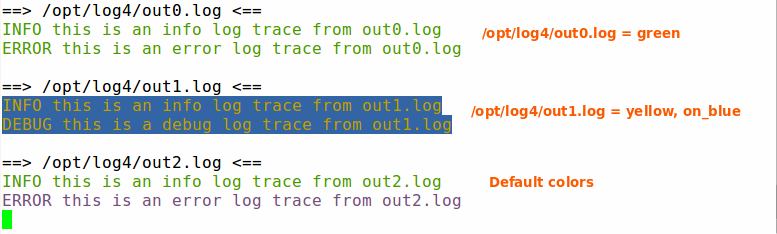
\includegraphics[scale=0.60]{multiple_colors.png}
\caption{\logftailer{} each log with its own color scheme}\label{fig:multiple_colors}
\end{figure}

\subsection{Filter Notification}
\label{sec:filter}
With filter you can filter out information you don't want to be printed out 
in the standard output. It would be a mix of tail and grep. You tail the log 
and grep for the information you are interested in. In order to enable that 
feature you need to execute \logftailer{} with the -f option:

\begin{cmd}
  ./log4tail -f[--filter] tracetofilter pathToLogs
\end{cmd}

\subsection{CornerMark Notification}
\label{sec:cornermark}
CornerMark notification will display a colored box in the bottom right side of
the terminal in case a Fatal, Error, Warning or Target trace has been found during the specified
time. In order to activate this type of notification you need to pass the
option cornermark in the command line as follows:

\begin{cmd}
  ./log4tail --cornermark numberofseconds pathToLogs
\end{cmd}
where numberofseconds can be any number. 

Example of what you would see if that notification is activated can be seen in
 \autoref{fig:cornermark}.

\begin{figure}[ht]
\centering
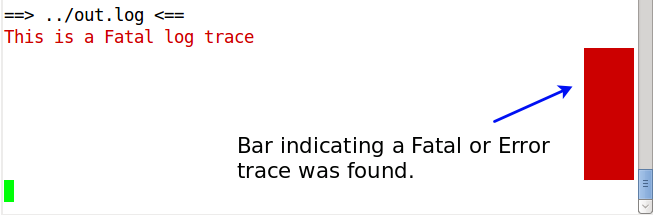
\includegraphics[scale=0.60]{terminalcornermark.png}
\caption{\logftailer{} with cornermark activated}\label{fig:cornermark}
\end{figure}

For Fatals and Errors the mark will be red. For Warnings will be yellow and for Targets 
will be cyan. These three colors are fine for easy identification in either clear terminal
backgrounds or dark ones.

The motivation for having a corner mark is when you need to go for a break and
want some kind of visual alert when something goes wrong. The visual alert will
be displayed for the number of seconds you specify in the command line, so it
is always advisable to be a number greater than the number of seconds you'll be
out of your desktop. 

\subsection{Mail Notification}
\label{sec:mailnotification}
\logftailer{} has an SMTP email client built-in if you want to be notified by email.
Mail notification is used when you want to be notified by email when a target or level (error or fatal) has been found 
in the logs. It is very useful when you are tailing for long hours and you cannot take 
a look at the screen from time to time. It's not necessary to run in silent mode anymore 
to use this action.
This action can be triggered by specifying the command line option -m and
specifying the mail details in a configuration file. 

\begin{cmd}
 ./log4tail -m [--mail] -c [--config] [[-t [--targets] 'regex1,...,regexN'] pathToLogs
\end{cmd}

\textbf{You'll need to provide a configuration file} with the following key parameters:

\begin{config}
\begin{verbatim}
 mail_username = yourusername
 mail_hostname = youremailhostname 
 mail_port = port
 mail_ssl = True or False
 mail_from = Email from, it can be the same as your to address 
 mail_to = Email to where you will receive the alerts
\end{verbatim}
\end{config}

\noindent
The password will be asked during runtime to avoid being left in plain ascii in
the configuration file. For SSL connection you will need a Python 2.6 runtime,
otherwise mail\_ssl should be left to False.

If an alert is raised, you will receive an email from mail\_from with the
subject ``Log4tailer alert'' for easy filtering.

\logftailer{} works with SMTP Google email accounts\footnote{Using SMTP SSL
connection. For SMTP SSL connectivity you'll need a Python 2.6 runtime, as
Python 2.4 does not support it.} if you have one.  In \autoref{fig:mailalert}
you can see how it looks like.

\begin{figure}[hb]
%\centering
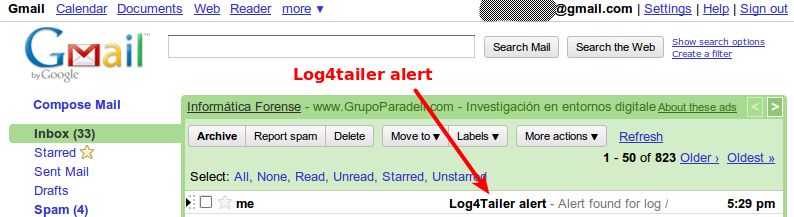
\includegraphics[scale=0.55]{emailalert.png}
\caption{\logftailer{} email alert in gmail}\label{fig:mailalert}
\end{figure}

I have not tested \logftailer{} with \textbf{sendmail}. For that you would have
to configure sendmail to accept smtp localhost connections.  Explaining that is
out of the scope of this document. You can take a look in the sendmail
documentation book in the Sendmail Consortium webpage at
\href{http://www.sendmail.org}{http://www.sendmail.org}.

\subsubsection{Flood control}
In order to avoid being sent lots of notification emails when a flood of
undesirable log traces turn up, log4tailer has a way to control that by means
of a 60 second gap, which means that non desirable levels that happen within
that gap are not notified. After that expiration time, the first undesirable
log trace to be found will be notified, triggering again a 60 second gap
period. 
 
\subsubsection{When should I use Mail notification}

MailAction would be like having additional eyes taking a look at the logs. That
means, that you can take a rest from time to time basically. If something is
found, then you are notified. At this stage, it will notify errors and fatals,
considered to be non desired levels in an application. Along with that, you can
specify a series of patterns (regexes), log4tailer's targets, that if found
could mean that the application is not behaving as expected. In that specific
case, you will get notified as well.
  
\subsection{Inactivity Notification}
\label{sec:inactivitysection}
Inactivity monitors for inactivity time in the logs. Inactivity as of this
release will just send an emphasized line in the standard output notifying that
there has been a lot of inactivity in that log. The inactivity time must be
provided in the command line with the -i parameter followed by the number of
seconds of inactivity to be monitored in the log.  If there has not been any
activity for the number of seconds given, \logftailer{} will print an
emphasized line in the standard output.\\ 
As an example:\\
\emphlogtrace{{Inactivity in the log for 5.99955296516 seconds}}
 
The command line interface to activate the inactivity monitoring is:
\begin{cmd}
 ./log4tail -i [--inact] numberinseconds pathToLogs
\end{cmd}

\subsubsection{Inactivity Mail Notification}
If you want a notification by email when inactivityAction is raised, just specify in the 
config file:

\begin{config}
\begin{verbatim}
 inactivitynotification = mail
\end{verbatim}
\end{config}

\noindent
By default is notification to the standard output as shown before. 

\subsection{Executor}
\label{sec:executor}

The executor is another type of notification. \logftailer{} will execute a
program provided by the user if the levels Error, Fatal or Critical have been
found in the log trace. The user must provide the command line option
\emph{--executable} along with a config file specifying the key \emph{executor}
with value the program you want log4tailer to execute and its parameters
separated by whitespaces. You can specify a couple of place holders as well,
where the first will be the log trace found and the second the log path where
the trace was found.

\begin{cmd}
 ./log4tail --executable -c configfile pathToLogs
\end{cmd}

where in configfile you could write something like:

\begin{verbatim}
 executor = anyscript %s %s 
\end{verbatim}

Where anyscript can be any program accepting two parameters, namely, lograce and log path. The script 
you provide, of course, will need to have execution permissions for the user 
owning the \logftailer{} process. 

As a simple example, if you cannot configure SMTP for log4tailer, then you could 
setup a script to use the \emph{mail} linux command line to send you an email by means of sendmail.

\subsection{Poster notification}
\label{sec:poster}
The poster notification is basically a REST client built in \logftailer{}. That will open 
the possibility to communicate with a centralized web server with a frontend. Poster 
notification will register to the server and notify all those fatal, critical, errors or 
targets found in the log. 
\begin{cmd}
 log4tail --post -c configfile.txt pathToLogs
\end{cmd}
where in the configfile.txt you will need to specify the following parameters:

\begin{config}
\begin{verbatim}
 server_url = url to the server
 server_port = port
 server_service_uri = /where/go/notifications
 server_service_register_uri = /register/log4tailer/toserver
 server_service_unregister_uri = /unregister/log4tailer/fromserver
\end{verbatim}
\end{config}

Upon unregistration, the server will delete the log from the database and all its related 
logtraces. So, if you don't want that happen, just point the unregister uri to a non existent one, 
and the server will not do anything, although it will keep the log as registered. Please, take a 
look at \autoref{sec:log4server}.

\subsection{PrintShot}
\label{sec:PrintShot}
The PrintShot notification is basically the Print notification adding the
capability of taking an screenshot whenever we find an alertable log trace. An
alertable log trace is any trace within levels Critical, Fatal and Error or
those that are targetable. In order to activate this notification, you need to
execute \logftailer{} in the following manner:

\begin{cmd}
 log4tail --screenshot -c configfile.txt pathToLogs
\end{cmd}

Where in the configfile.txt you should specify the following key:

\begin{config}
screenshot = fullpathtopicture.png
\end{config}

\subsubsection{requirements}
The PrintShot notification requires you have the \textbf{import} command line
program to take screenshots. So, make sure you have that software installed.
Most modern Linux distributions have it. 

\subsubsection{When should I use this feature}
This feature is useful whenever you are testing in your local desktop any
software and you would like to have a proof that some log trace is getting
traced by that software. It would be good for software documentation purposes
as well. 

\section{Pause Modes}
\label{sec:PauseModes}
As of release 1.2 \logftailer{} includes pausemodes feature. You will be able
to pause or freeze the output by a number of seconds if an specific level or
target has been found. In order to enable pausemodes, you must configure them
in a config file providing any of the following keys\footnote{the keys are case
insensitive, so is the same pauseDEBUG or pausedebug\ldots} :

\begin{config}
\begin{verbatim}
 pausedebug = secondsfordebug
 pauseinfo = secondsforinfo
 pausewarn = secondsforwarn
 pauseerror = secondsforerror
 pausefatal = secondsforfatal
 pausetarget = secondsfortarget
\end{verbatim}
\end{config}

\noindent
You specify only those ones you want to use.
For instance, if we want to freeze the output momentarily (one second) for warnings:

\begin{config}
\begin{verbatim}
 pausewarn = 1
\end{verbatim}
\end{config}

\noindent
Then, we should run log4tailer like:
\begin{cmd}
./log4tail -c yourconfig /pathToLogs
\end{cmd}
Pausetarget keyword will pause the output for any regex found in the log when
running log4tailer with -t option.

\section{Reporting}
Every time we finish the tailing, log4tailer will output a report, specifying
how long log4tailer has been running and the number of events for debug, info
and warn. In case of error and fatal, it will provide the timestamps when they
were found and their corresponding logtrace.  Example:

\begin{verbatim}
Analytics: 
Uptime: 
0.0 years 0.0 days 0.0 hours 0.0 mins 45.9482619762 secs 
Report for Log out.log
Levels Report: 
FATAL:
ERROR:
15 May 2009 17:17:43=>> There was an error here
15 May 2009 17:17:44=>> There was another one in here
15 May 2009 17:17:45=>> Oops, another one
WARN:
4
INFO:
9
DEBUG:
14
TARGET:
3
OTHERS:
18 Jul 2010 11:45:44=>> Inactivity action detected
Ended log4tailer, because colors are fun
\end{verbatim}

\subsection{Reports by email}
If you want a report by email after a given amount of time, then you can do
that by means of the config file. There are two values that can be setup,
namely:

\begin{config}
\begin{verbatim}
 analyticsnotification = mail
 analyticsgaptime = 10.5
\end{verbatim}
\end{config}

If these two values are uncommented, then you will be required to provide the
mail details in the same configuration file, please check the
\autoref{sec:mailnotification}. The analyticsgaptime should be given in
seconds, by default is 3600 seconds (1 hour).  You'll receive a report after
that period. After that period the statistical information is flushed and then
sent again once the gap notification time is expired and so on.  In
\autoref{fig:emailnotification} %in page \pageref{fig:emailnotification}, you
can see an email report notification in a Google gmail account.

\begin{figure}[ht]
%\centering
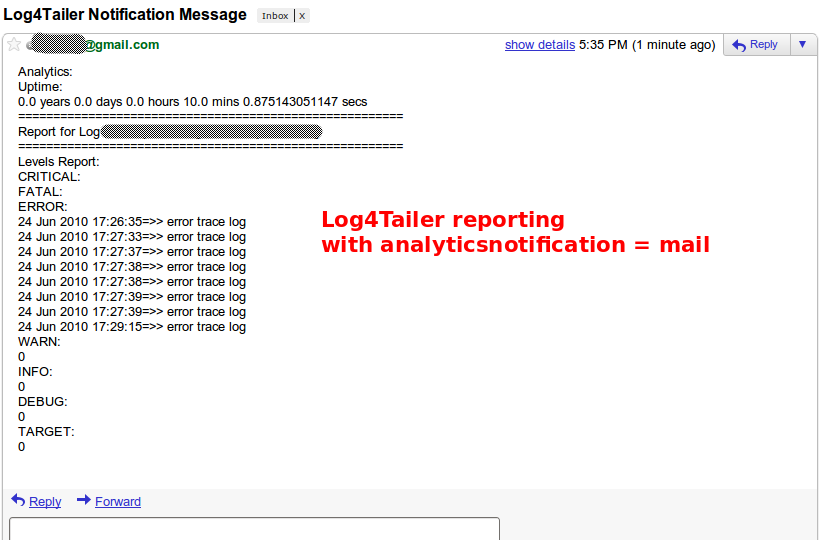
\includegraphics[scale=0.50]{emailnotification.png}
\caption{\logftailer{} email report notification}\label{fig:emailnotification}
\end{figure}

\subsection{Reports to a file}
\logftailer{} can give you a report to a file if you want to. Just provide the
analyticsnotification in the configuration file pointing to the reporting file
(full path). An example of that would be:

\begin{config}
\begin{verbatim}
 analyticsnotification = /opt/reportlog4tailer.txt
 analyticsgaptime = 10.5
\end{verbatim}
\end{config}

\section{Silent Mode}
Silent mode, tails the logs in the background (daemonized tailer) and triggers
the Mail notification, notifying if error, fatal or any target has been found
in the logs. 

The syntax to activate the silent mode is:
\begin{cmd}
 ./log4tail -s -c [--config] configfile [-t [--targets] 'regex1,..,regexN'] fullPathToLogs
\end{cmd}

\logftailer{} will require a configuration file with your email details. Please
take a look at the \autoref{sec:mailnotification} where specifies the key
parameters that need to be specified. It is very important to note that the
path to the logs must be the full path, no relative. That's because when
\logftailer{} enters in daemonized mode, it switches to the root directory
closing all buffers and detaching itself from the terminal, in other words, it
becomes a real daemon. As a consequence, it is not necessary to execute it with
the nohup Linux command line tool.

\subsection{Silent Mode when no access to email notification}
\logftailer{} provides the no-mail-silence optional command line parameter,
where it enters in daemonized mode with no notification setup. It will be up to
the user to setup some type of notification by means of a configuration file.
Actually, this option is thought to be used along with the -config parameter
where you can specify some notification. One of the scenarios would be when you
want automatic monitoring when the server you are running \logftailer{} has no
ports available for email notification. You could provide a config file with
\emph{analyticsnotification} pointing to a file where \logftailer{} would do a
report of the logs status every \emph{analyticsgaptime} seconds or one hour by
default.

\begin{cmd}
 ./log4tail --no-mail-silence -c [--config] configfile fullPathToLogs
\end{cmd}


\section{Coloring Standard Input}
Log4tailer can colorize its standard input to the standard output. Main use
would be when your application does some output and finishes. In order to do
that just type:
\begin{cmd}
 yourapplication | log4tail -
 cat somelog.log | log4tail -
\end{cmd}
You can use the \emph{more} Linux/Unix application in order to page the output.
Example:
\begin{cmd}
 cat somelog.log | log4tail - | more
\end{cmd}

\section{Tailing last N lines}
You can tail last \emph{N} lines from the log with the \emph{-n} option. Just type:
\begin{cmd}
 ./log4tail -n numberOfLines pathToLog
\end{cmd}
and it will output the last \emph{numberOfLines} from the log colorizing the
corresponding levels.

\section{SSH Tailing}
SSH Tailing or remote tailing will allow you to tail multiple remote logs from
different hosts. As of now, only PrintAction is available, so you'll be able to
tail multiple remote logs in a colorful way as specified in section
\ref{sec:PrintAction}. In order to tail remotely you'll need to pass as a
parameter the -r option along with some config file parameters:

\begin{cmd}
 ./log4tail -r -t targets -c yourconfig.txt
\end{cmd}
In your configfile you must provide the following parameters:

\begin{config}
\begin{verbatim}
 sshhostnames = hostname0, hostname1, hostnameN-1
 hostname0 = username0, /var/log/log0, /var/log/log1, /var/log/logN-1
 hostname1 = username1, /var/log/log0, /var/log/log1, /var/log/logN-1
 hostnameN-1 = usernameN-1, /var/log/log0, /var/log/log1, /var/log/logN-1
\end{verbatim}
\end{config}

\noindent
Where:
\begin{itemize}
\item \textbf{sshhostnames} is a comma separated values of hostnames
\item every \textbf{hostname} must be a parameter itself where first 
value should be its username and then the logs you want to tail.
\end{itemize}

By default log4tailer will try to authenticate by using your rsa key under your
$\sim$/.ssh/id\_rsa key if it exists, otherwise it will use normal username, password
authentication. \textbf{Please be aware that you need to be the same username
in both client and server. So, if you are logging in as root the ssh key needs
to be for the root user. Otherwise, it would request your password}.
If you want to use another rsa key other than the default
id\_rsa key then you can provide one in the config file by using the rsa\_key
parameter. Example:

\begin{config}
\begin{verbatim}
 rsa_key = /home/youruser/.ssh/myrsakey
\end{verbatim} 
\end{config}

\noindent
rsa\_key value must be the full path to the rsa\_key.

Some considerations are to be taking into account. As of now, remote tailing
\textbf{only} provides PrintAction along with targets, that means that you will
be able to tail with colors and emphasize those log traces that match the comma
separated regexes provided with -t. Besides, you'll be able to use pauseModes
set up in the config file as explained in section \ref{sec:PauseModes}.

To finish, just Ctrl-c and it will close all channels opened to communicate to
the remote hosts. 

\subsection{Dependencies for SSH tailing}
It is very important to note that for remote tailing, you'll need to install
the \textbf{paramiko module}, available in major Linux distributions. In most
of them is available under the name of python-paramiko. In Debian systems,
you'll need to type:
\begin{cmd}
 sudo apt-get install python-paramiko
\end{cmd}

\section{Configuration file}
Config file is provided fully documented for convenience; just uncomment those
lines you are interested to enable and modify them for your specific purposes.
In order to enable those values in the config file, you must notify that to
\logftailer{} as a parameter in startup time.

\begin{cmd}
 ./log4tail -c yourconfig.txt logs
\end{cmd}
If you always use the same configuration file, you can copy it in your HOME
directory as \emph{.log4tailer} and log4tail will read it next time you execute
the program, even if you don't provide the -c option.

The config file provided for convenience is called log4tailerconfig.txt and is quoted below:

\begin{verbatim}

# Optional config for log4tailer
# to activate it
# log4tail -c config yourlogs

# ====================================================
# Custom colours for every level. Available 
# colours are: red, green, yellow, blue, magenta, cyan 
# and white. Uncomment to override the default ones.
# ====================================================

# warn = yellow, on_cyan
# error = magenta 
# fatal = red, on_green
# info = green
# debug = black

# ================================
# targets: which lines do you want 
# to emphasize by using regexes
# uncomment and provide your values.
# ================================

# targets path/to/log0 = regex0,regex1,regex2 | coloregex0, coloregex1, ...
# targets path/to/log1 = regex0,regex1,regex2 | coloregex0, coloregex1, ...

# ======================================================
# Every log with its own color scheme, overriding colors 
# for every level.
# ======================================================

# /path/to/log0 = yellow
# /path/to/log1 = red

# ======================================================
# Pause the output by the number of seconds specified if 
# a level or target has been found. Uncomment the ones 
# you want. The value can be any number in seconds. 
# ======================================================

# pausedebug = 4
# pauseinfo = 2
# pausewarn = 1
# pauseerror = 1
# pausefatal = 1
# pausetarget = 1

# ======================================================
# Mail details 
# ======================================================

# mail_username = yourhostusername
# mail_hostname = mailhostname
# mail_port = 25
# mail_ssl = True or False
# mail_from = any from address
# mail_to = alerts will be sent in the address you specify in here

# ===================================================================
# executor notification
# ===================================================================

# executor = program command1 command2 %s %s
# executor = program command1 command2 

# ===================================================================
# poster notification
# ===================================================================

# server_url = url to the server
# server_port = port
# server_service_uri = /where/go/notifications
# server_service_register_uri = /register/log4tailer/toserver
# server_service_unregister_uri = /unregister/log4tailer/fromserver

# ===================================================================
# Inactivity notification, by email or stdout.
# Possible values can be "mail" or "print". By default is "print".
# ===================================================================

# inactivitynotification = mail

# ====================================================================
# Analytics notification. You can make log4tailer send you 
# a report every analyticsgaptime seconds. By default it will be 
# printed out once finished. Uncomment analyticsnotification to 
# report by email or to a file. Another possible value can be "print".
# ====================================================================

# analyticsnotification = mail
# analyticsnotification = fullPathToaFile
# analyticsgaptime = 10.5

# ==============================
# SSH Tailing parameters
# ==============================

# sshhostnames = hostname0, hostname1, hostnameN-1
# hostname0 = username0, /var/log/log0, /var/log/log1, /var/log/logN-1
# hostname1 = username1, /var/log/log0, /var/log/log1, /var/log/logN-1
# hostnameN-1 = usernameN-1, /var/log/log0, /var/log/log1, /var/log/logN-1

# rsa_key defaults to ~/.ssh/id_rsa, if that's not your case then 
# provide yours

# rsa_key = fullpathToRsaKeyName 

\end{verbatim}

\newpage

\part{Log4Server}

\section{A centralized reporting web application}
\label{sec:log4server}
The \logftailer{} project includes a web backend application that receives
notifications from the log4tailer clients, notifying in a web front page about
the status of the logs in several machines. The log4server is implemented using
the Django web framework and can run in any wsgi compliant web server, such as
Apache, Cherokee, Nginx or CherryPy, just to name a few. Basically, the clients
will register first to the server and then notify if any fatal, error, critical
or target logtrace has been found. 

A network diagram is showed in \autoref{fig:serverdiagram}.

\begin{figure}[hb]
\centering
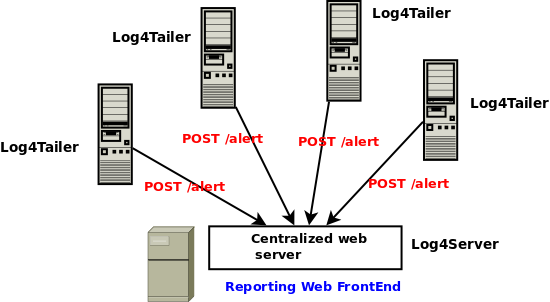
\includegraphics[scale=0.50]{serverdiagram.png}
\caption{Log4Server network diagram}\label{fig:serverdiagram}
\end{figure}


In the next section, we will describe the API that the log4server application
implements and the one being used by the log4tailer poster notification.

\section{Log4Tailer compliant server}
\logftailer{} client has the poster notification that allows the tailer to
communicate with a centralized web application, notifying it of possible
problems from remote logs.  The poster notification will first register the
tailer client to the server, and next calls will be for alert notifications
only.

\subsection{Log4Tailer server API REST interface}

The compliant API interface is as follows:

\subsubsection{Registration}

Log4tailer client registers to the server on startup when poster notification
is provided.

\begin{flushleft}
 \begin{tabular}{|c|c|l|}
 \hline 
 \rowcolor{cyan} {\color{white} \textit{\textbf{HTTP Method}}} &  {\color{white} 
  \textit{\textbf{URL}}}  & {\color{white} 
 \textit{\textbf{Description}}}\\
 POST & /register/ & Log4tailer client registration to the server\\
 \hline
\end{tabular}
\end{flushleft}
The POST method will have in the body a JSON object with the following
information:

\begin{itemize}
 \item logpath Full path of the log 
 \item hostname log's server hostname
\end{itemize}

\noindent
Upon a successul POST the server will reply a 201 CREATED answer.

\noindent
Example:

\begin{codeexample}

POST /register/

 \{``logpath'' : ``/var/log/messages'', ``logserver'' : ``localhost''\} 

RESPONSE

 \{``id'' : 3\} 

HTTP/1.1 201 CREATED.
\end{codeexample}

The id returned is the log identifier id.

\subsubsection{Unregistration}

Log4tailer client unregisters from the server ones it is stopped.

\begin{flushleft}
 \begin{tabular}{|c|c|l|}
 \hline 
 \rowcolor{cyan} {\color{white} \textit{\textbf{HTTP Method}}} &  {\color{white} 
  \textit{\textbf{URL}}}  & {\color{white} 
 \textit{\textbf{Description}}}\\
 POST & /unregister/ & Log4tailer client unregistration to the server\\
 \hline
\end{tabular}
\end{flushleft}
The POST method will have in the body a JSON object with the following
information:

\begin{itemize}
 \item id log registration id 
\end{itemize}

\noindent
Upon a successul POST the server will reply a 200 OK answer

\noindent
Example:

\begin{codeexample}

POST /unregister/

 \{``id'' : 4 \}

RESPONSE

HTTP/1.1 200 OK.
\end{codeexample}

\subsubsection{Alerting}

\begin{flushleft}
 \begin{tabular}{|c|c|l|}
 \hline 
 \rowcolor{cyan} {\color{white} \textit{\textbf{HTTP Method}}} &  {\color{white} 
  \textit{\textbf{URL}}}  & {\color{white} 
 \textit{\textbf{Description}}}\\
 POST & /alerts/ & New alert has been found.\\
 \hline
\end{tabular}
\end{flushleft}
The POST method will have in the body a JSON object with the following
information:

\begin{itemize}
 \item logtrace logtrace that triggered the alert.
 \item level level of the aforementioned logtrace.
 \item log log where the logtrace belongs to.
    \begin{itemize}
      \item logpath Full path of the log 
      \item hostname log's server hostname
    \end{itemize}
\end{itemize}
Upon a successul POST the server will reply a 201 CREATED answer.

\noindent
Example:

\begin{codeexample}

POST /alerts/

 \{``logtrace'' : ``This is an error trace'', 
   ``loglevel'' : ``error'',
   ``log'' : \{``id'' : ``logid'', ``logpath'' : ``/var/log/messages'', ``logserver'': 
``192.168.1.1''\}\} 

RESPONSE

HTTP/1.1 201 CREATED.
\end{codeexample}

\subsubsection{Status}

\begin{flushleft}
 \begin{tabular}{|c|c|l|}
 \hline 
 \rowcolor{cyan} {\color{white} \textit{\textbf{HTTP Method}}} &  {\color{white} 
  \textit{\textbf{URL}}}  & {\color{white} 
 \textit{\textbf{Description}}}\\
 GET & /alerts/status & Status of the log files.\\
 \hline
\end{tabular}
\end{flushleft}
It returns all log traces triggered along with the log and server they belong
to. The date when it happened is reported as well. The results are paginated in
reverse order, the newest first.

\noindent
Example:

\begin{codeexample}

GET /alerts/status

RESPONSE

HTTP/1.1 200 OK.
\end{codeexample}


\noindent
If you go to /alerts/status in your web browser, you would see something as
showed in  \autoref{fig:logstatus}.

\begin{figure}[ht]
%\centering
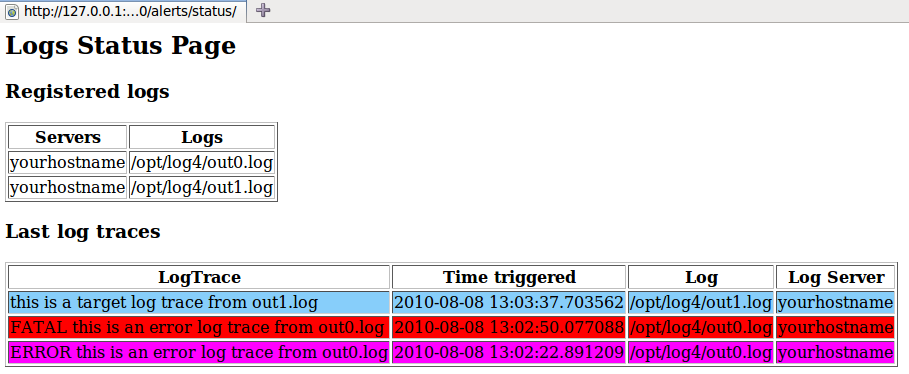
\includegraphics[scale=0.50]{logstatus.png}
\caption{Log4Server status web reporting}\label{fig:logstatus}
\end{figure}

\section{Log4Server deployment}
Log4Server is implemented using the Django web framework. It persists alertable
log traces into a database for easy reporting and log4tailer client
registrations. 

The application uses buildout to manage all application dependencies and
deployment. By issuing the bin/buildout command, it will build a
log4server.wsgi file, that is the one that you will need to use when setting up
the web server. In this document, we will show the instructions on how to set
it up by using the Apache web server. 

\subsection{Building the wsgi file}

First of all, download the log4server distribution sources from googlecode
site. Untar the package and execute\footnote{The project provides a Makefile
that executes the bin/buildout command for convenience. It can take a while, so 
relax and take a cup of tea.}:

\begin{cmd}
    virtualenv --no-site-packages ENV
    . ENV/bin/activate
    python bootstrap.py
    bin/buildout
\end{cmd}

If everything is fine\footnote{You need external internet connectivity, as it
will download all dependencies such as Django web framework in the current
directory.} you will see a directory called \emph{bin}. If you go
into that directory you will see a file called log4server.wsgi. 

\subsection{Apache configuration}
In a Debian system such as Ubuntu, you'll need to install Apache and
libapache2-mod-wsgi. Once installed, proceed as follows:

\begin{cmd}
    cd /etc/apache2/sites-available
\end{cmd}
and place a file called log4tailer.conf with the following
contents\footnote{this Apache2 configuration has been tested on an Ubuntu
Maverick 10.10 Server}:

\begin{config}
\begin{verbatim}

Listen 127.0.0.1:8000

Alias /media/ /path\_to\_log4server-version/src/log4server/media/

<VirtualHost *:8000>
    WSGIDaemonProcess log4server processes=1 threads=5 display-name=%{GROUP}
    WSGIProcessGroup log4server
    WSGIScriptAlias / /path\_to\_thewsgi/log4server/bin/log4server.wsgi
</VirtualHost>

WSGISocketPrefix     run/wsgi
WSGIRestrictStdout   off

\end{verbatim}
\end{config}

Then, go to:

\begin{cmd}
    cd /etc/apache2/sites-enabled
\end{cmd}
and place a soft link to the previous created log4tailer.conf file:

\begin{cmd}
    ln -s ../sites-available/log4tailer.conf
\end{cmd}

\subsection{Deciding on database}

Log4Server needs a database in order to persist the alertable logtraces. 
Sqlite3, Mysql or PostGres should be, by far, enough. Actually, with just an
Sqlite3 would be just fine. Before starting the server, you should
sync the database the first time or any time that the database does not exist
already. In order to do that, execute the following command:

\begin{cmd}
   bin/log4server syncdb 
\end{cmd}
\emph{log4server} is just a wrapper for the \emph{manage.py} Django python
script. 

\subsection{Restarting Apache}
Once you have placed the Apache configuration file pointing to the wsgi file, 
you'll need to restart Apache. 

\subsection{Main Web Frontend urls}
Once Apache is running, open a web browser and go to the next url to see if it
works:

\begin{codeexample}
http://hostname:port/alerts/status
\end{codeexample}

If you see a web page with the title \textbf{Logs Status Page} then it means
it's working. Congratulations!!. 


\newpage

\part{Case Studies}
\section{Full Automatic Log Monitorization}
Full Automatic log monitorization can be performed when you execute \logftailer{} 
in silent mode passing the parameters \emph{-s}. 
Log4Tailer will run silently in the background notifying by email 
when something goes wrong. As of now, it will notify errors, fatals and those targets 
specified as a parameter or in the config file. It is important to notice that every log 
can have its own set of targets (regexes). Apart from that, you can make log4tailer 
to monitor inactivity in the log and notify you by email as well. You just need to specify 
that in the config file as explained in the section \ref{sec:inactivitysection}.

Summing up, full automatic monitorization will monitor inactivity, errors, fatals and targets specified 
in the config file or command line as parameters. This will give you extra confidence on the 
monitoring of your application if your application uses already nagios or other monitoring software.
\footnote{It is important to notice that pausemodes should not be enabled. That feature is 
to pause the output when having PrintAction enabled.}

\section{Semi Automatic Log Monitorization}
You can have a mix of email notification and normal colorized print action. You just 
need to execute log4tailer passing as a parameter \emph{-m} and the 
corresponding configfile if you want to enable additional features. 

\section{No SMTP email access for log4tailer}
Sometimes a server can have the email ports closed (firewalled) due to security policies. 
Alternatives:
\begin{itemize}
\item For those cases you can use the executor notification using the mail Linux command line to 
send email provided that the server runs some 
kind of MTA like sendmail. Let's see an example:
\begin{cmd}
 log4tail --executable -c configfile.txt /var/log/out.log
\end{cmd}
where in the configfile.txt you could write something like\footnote{If you use the 
\emph{echo} command line tool providing both place holders (log trace, log path), make 
sure you leave a white space in between quotes.}:
\begin{verbatim}
 executor = echo ' %s %s ' | mail -s 'log4tailer alert' -t youremail@hostname.com
\end{verbatim}
If sendmail sends email to your localhost, then you could read the email easily by using the 
famous command line client mutt for example. It's important to note, that you can daemonize 
\logftailer{} in that case as well:
\begin{cmd}
 log4tail --no-mail-silence --executable -c configfile.txt /var/log/out.log
\end{cmd}
That means that log4tailer will be a daemon monitoring the out.log and sending email by using 
the mail Linux command line. 

\item You can always make \logftailer{} to report you in a file every some minutes or 
activate the cornermark notifications (see section \ref{sec:cornermark}). 
Both features are really nice to activate them when 
you need to go for a break. You can setup the cornermark feature with the \emph{cornermark}
parameter specifying a time in seconds bit longer than the time you'll be out of your desktop
to avoid the mark going away. The marks stay in the terminal for the time you specify.
\end{itemize}


\newpage

%\part{Development}
\section{Hacking}
If you would like to collaborate, just let me know. I'm taking this project seriously now and 
any new feature will require unit testing. This project was originally a multicolored tailer and I just 
did not bother about unit testing as it was short in code and did basically what I wanted. This project is 
going to grow significantly and I just do not want to break any functionality that already works. As of this 
release I've been using unittest and mox (mocking) libraries. 

\logftailer{} began in launchpad, but as I was working on my own, I moved it to googlecode. If more people joins 
in this project, it could be moved to launchpad, as it is more suited for bigger opensource teams.

\section{Class Diagram}
In the next figure we can take a look at what is the relationship between classes in the log4tailer 
project:

\begin{figure}[htp]
\centering
\includegraphics[scale=0.60]{log4tailerClassDiagram.png}
\caption{\logftailer{} class diagram}\label{fig:class diagram}
\end{figure}



\section{Further work\footnote{work that could or could not be implemented in future releases.}}

\logftailer{} began being just a multicolored tailer, but it has been growing in functionalities and new 
concepts. With the introduction of \emph{Actions}, \logftailer{} can be expanded to use more functionalities. 
Features that I've been thinking of:
\begin{enumerate}
 \item web frontend action
 \item ncurses action
 \item nagios action
\item \emph{Analytics} will introduce log behaviour analysis based on patterns and log statistical analysis.
 \item \emph{Log4Servers} and \emph{Log4Clients} will enable having log4tailers being run in remote servers and clients 
will be able to communicate to those servers and trigger a decission based on the log4tailers action outcomes.
\item tailing remotely from your desktop by means of ssh.
\item Inactivity action could notify by using other actions like emailing. As of now it uses printing. Actually, 
inactivity monitoring is not a notification action, so maybe I'll make a package for monitoring stuff to 
separate the concept of notification actions vs monitoring actions.
\item I'll write an optional installer to install \logftailer{} system wide, but you will be able to run it 
in standalone mode.
\item A GTK gui
\end{enumerate}
\newpage

%\printindex
\end{document}
